\documentclass[tikz,border=6pt]{standalone}
\usepackage{amsmath,amssymb}
\usepackage{xcolor}
\definecolor{accent}{HTML}{A13D2C}
\definecolor{accent2}{HTML}{2B5F6B}
\definecolor{muted}{HTML}{5A564F}
\definecolor{linecol}{HTML}{D8D2C4}
\definecolor{astroblue}{HTML}{1B4F72}
\definecolor{sunyellow}{HTML}{E8A33D}
\usetikzlibrary{calc,arrows.meta,angles,quotes}
\usepackage[T1]{fontenc}\usepackage{newpxtext,newpxmath}  % same fonts as the notes
\begin{document}
% Galactic disk seen from the north Galactic pole, to scale: R0 = 8.2 kpc, l = 30 deg.
% x from the Sun toward the centre, y toward l = 90 deg (direction of rotation at the Sun).
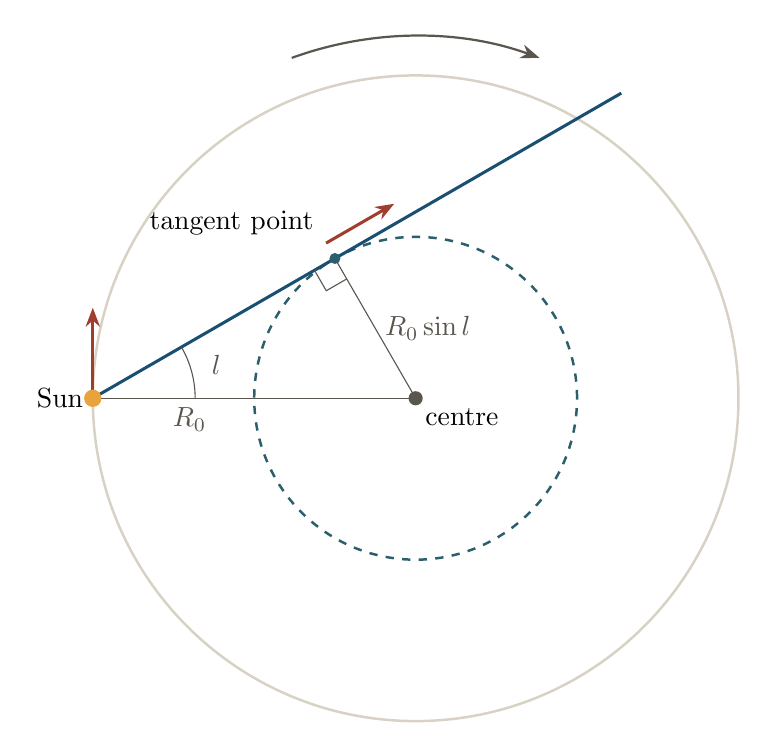
\begin{tikzpicture}[x=0.5cm,y=0.5cm, >={Stealth[length=2.4mm]}]
  \coordinate (C) at (0,0);
  \coordinate (S) at (-8.2,0);
  \coordinate (T) at ({-8.2+8.2*cos(30)*cos(30)},{8.2*cos(30)*sin(30)});
  \coordinate (E) at ({-8.2+15.5*cos(30)},{15.5*sin(30)});
  \draw[linecol, line width=0.9pt] (C) circle (8.2);
  \draw[accent2, dashed, line width=0.9pt] (C) circle (4.1);
  \draw[muted] (S) -- (C) node[pos=0.3, below] {$R_0$};
  \draw[muted] (C) -- (T) node[midway, right] {$R_0\sin l$};
  \draw[astroblue, line width=1.1pt] (S) -- (E);
  \pic[draw, muted, angle radius=1.3cm, "$l$", angle eccentricity=1.25] {angle = C--S--E};
  \pic[draw, muted, angle radius=0.3cm] {right angle = C--T--S};
  % velocities on circular orbits (no labels)
  \draw[->, accent, line width=1.1pt] (S) -- ++(0,2.3);
  \draw[->, accent, line width=1.1pt] ($(T)+({-0.45*sin(30)},{0.45*cos(30)})$) -- ++({2.0*cos(30)},{2.0*sin(30)});
  % sense of rotation
  \draw[->, muted, line width=0.8pt] ([shift={(110:9.2)}]C) arc (110:70:9.2);
  \fill[sunyellow] (S) circle (0.22);
  \fill[muted] (C) circle (0.18);
  \fill[accent2] (T) circle (0.14);
  \node[left] at (S) {Sun};
  \node[below right] at (C) {centre};
  \node[anchor=south east] at ($(T)+(-0.3,0.35)$) {tangent point};
\end{tikzpicture}
\end{document}
